\chapter{วิศวกรรมการหมักและเทคโนโลยีการผลิตปุ๋ยชีวภาพระดับอุตสาหกรรม}
\label{ch:biofertilizers}

\begin{keyconcept}[แนวคิดสำคัญของบทที่ 6]
ปุ๋ยชีวภาพ (Biofertilizers)\index{ปุ๋ยชีวภาพ (Biofertilizers)} คือชีวภัณฑ์ที่บรรจุเซลล์จุลินทรีย์มีชีวิตที่มีความสามารถเฉพาะเจาะจงในการตรึงไนโตรเจน การละลายฟอสฟอรัสและโพแทสเซียม หรือการกระตุ้นการดูดซึมธาตุอาหารของรากพืช การขยายขนาดการผลิตจากระดับห้องปฏิบัติการสู่ระดับอุตสาหกรรมจำเป็นต้องอาศัยศาสตร์ด้าน \textbf{วิศวกรรมการหมัก (Fermentation Engineering)\index{วิศวกรรมการหมัก (Fermentation Engineering)}} การควบคุมจลนศาสตร์การเพาะเลี้ยงแบบกะ (Batch) และกะกึ่งต่อเนื่อง (Fed-batch) การถ่ายโอนมวลออกซิเจน ($k_L a$)\index{สัมประสิทธิ์การถ่ายโอนออกซิเจน ($k_L a$)}\index{Oxygen transfer coefficient ($k_L a$)} ตลอดจนเทคโนโลยีการห่อหุ้มเซลล์ (Microencapsulation)\index{การห่อหุ้มเซลล์ระดับไมโคร (Microencapsulation)} ด้วยวัสดุพาหะชีวภาพ เช่น ถ่านไบโอชาร์และโซเดียมอัลจิเนต เพื่อรักษาความมีชีวิตของเซลล์ตามเกณฑ์มาตรฐาน พ.ร.บ. ปุ๋ย กรมวิชาการเกษตร\index{พ.ร.บ. ปุ๋ย กรมวิชาการเกษตร}
\end{keyconcept}

\begin{figure}[ht]
    \centering
    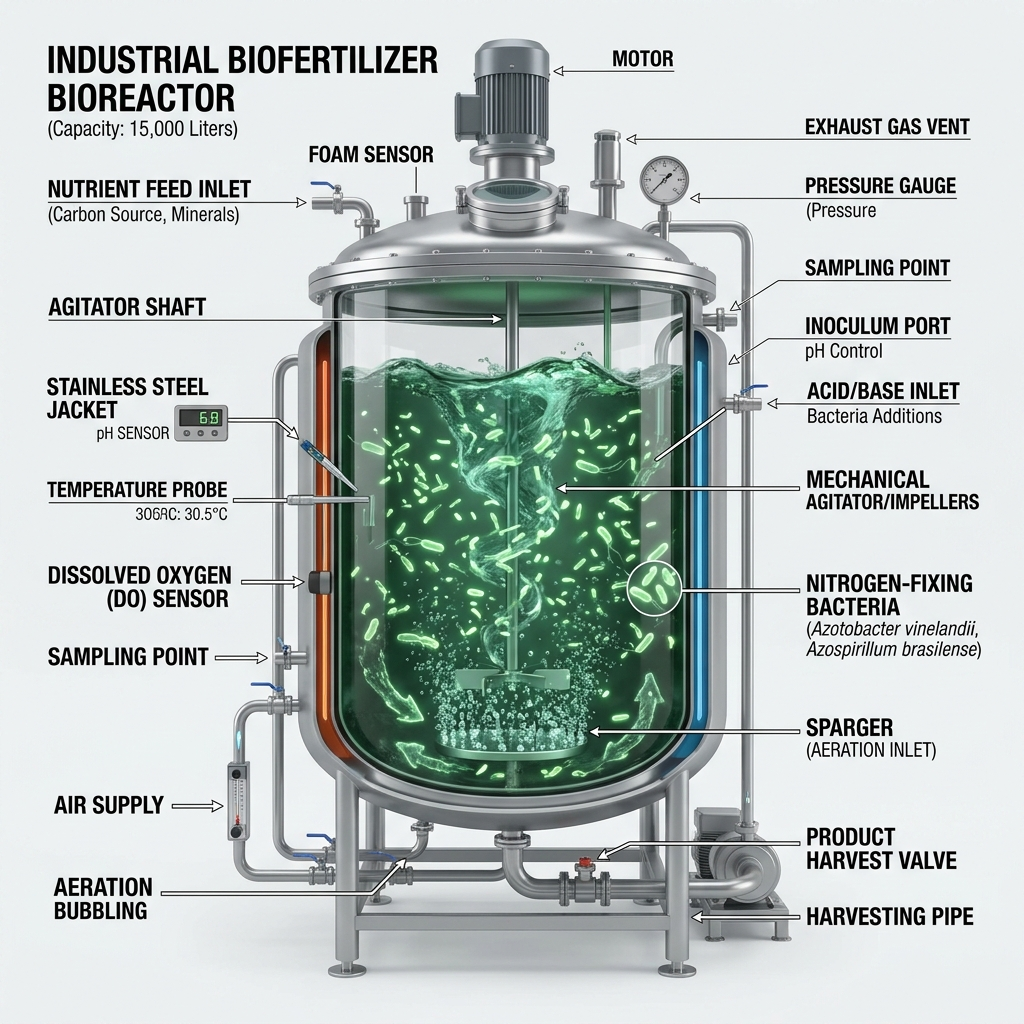
\includegraphics[width=0.85\textwidth]{assets/ch06_biofertilizer_fermentation.png}
    \caption{การจำลอง 3D ของเครื่องปฏิกรณ์ชีวภาพกวนสมบูรณ์ (Stirred-Tank Bioreactor) ขนาดกึ่งอุตสาหกรรม แสดงระบบจ่ายอากาศอัด (Sparger) ใบพัดกวนแบบ Rushton turbine เซนเซอร์วัดออกซิเจนละลายน้ำ (DO) และหัววัดกรด-ด่าง (pH) สำหรับการเพาะเลี้ยงแบคทีเรียปุ๋ยชีวภาพความหนาแน่นสูง}
    \label{fig:ch06_biofertilizer_fermentation}
\end{figure}

\section*{วัตถุประสงค์การเรียนรู้ประจำบท}
เมื่อศึกษาบทเรียนนี้จบแล้ว นักศึกษาสามารถ:
\begin{enumerate}
    \item จำแนกชนิดของปุ๋ยชีวภาพตามหน้าที่ทางชีวภาพและกลไกการปลดปล่อยธาตุอาหาร
    \item วิเคราะห์หลักการวิศวกรรมชีวภาพในการเพาะเลี้ยงเซลล์ความหนาแน่นสูง และการวัดสัมประสิทธิ์การถ่ายโอนมวลออกซิเจน ($k_L a$)
    \item เปรียบเทียบจลนศาสตร์การเพาะเลี้ยงแบบกะ (Batch) แบบกะกึ่งต่อเนื่อง (Fed-batch) และแบบต่อเนื่อง (Continuous)
    \item อธิบายเทคโนโลยีการตรึงเซลล์และการห่อหุ้มเซลล์ (Microencapsulation) ด้วยโซเดียมอัลจิเนตและวัสดุพาหะถ่านชีวภาพ (Biochar)
    \item ประเมินคุณภาพปุ๋ยชีวภาพตามเกณฑ์มาตรฐานกฎหมาย พ.ร.บ. ปุ๋ยของกรมวิชาการเกษตร และคำนวณปริมาณเซลล์มีชีวิต (CFU)
\end{enumerate}

\section{การจัดหมวดหมู่และกลไกสรีรวิทยาของปุ๋ยชีวภาพ}

ปุ๋ยชีวภาพจัดจำแนกตามคุณสมบัติการปลดปล่อยธาตุอาหารแก่พืชออกเป็น 4 กลุ่มหลัก:

\subsection{1. ปุ๋ยชีวภาพตรึงไนโตรเจน (Nitrogen-Fixing Biofertilizers)}
\begin{itemize}
    \item \textbf{กลุ่มพึ่งพาอาศัยในปมราก (Symbiotic):} แบคทีเรียสกุล \organism{Rhizobium}\index{Rhizobium@\textit{Rhizobium}}, \organism{Bradyrhizobium}\index{Bradyrhizobium@\textit{Bradyrhizobium}}, และ \organism{Sinorhizobium} สำหรับพืชตระกูลถั่ว สามารถตรึงไนโตรเจนได้สูงถึง $100 - 300\text{ kg N/ha/ปี}$
    \item \textbf{กลุ่มอยู่ร่วมกันแบบพึ่งพาภายนอก (Associative Symbiosis):} แบคทีเรียสกุล \organism{Azospirillum}\index{Azospirillum brasilense@\textit{Azospirillum brasilense}} (เช่น \organism{A. brasilense}) อาศัยบริเวณผิวรากและช่องว่างระหว่างเซลล์คอร์เทกซ์ของพืชตระกูลหญ้า ข้าว ข้าวโพด และอ้อย ตรึงไนโตรเจนได้ $20 - 50\text{ kg N/ha/ปี}$ พร้อมหลั่งฮอร์โมน IAA
    \item \textbf{กลุ่มดำรงชีวิตอิสระในดิน (Free-Living):} แบคทีเรียสกุล \organism{Azotobacter}\index{Azotobacter chroococcum@\textit{Azotobacter chroococcum}} (เช่น \organism{A. chroococcum}) และ \organism{Beijerinckia} ตรึงไนโตรเจนในสภาวะมีออกซิเจนโดยอาศัยกลไก Respiratory Protection
    \item \textbf{กลุ่มไซยาโนแบคทีเรีย (Cyanobacteria):} \organism{Anabaena azollae}\index{Anabaena azollae@\textit{Anabaena azollae}} ที่อาศัยในโพรงใบของแหนแดง (\organism{Azolla}) นิยมปล่อยลงในนาข้าวเพื่อเป็นปุ๋ยพืชสดไนโตรเจนสูง
\end{itemize}

\subsection{2. ปุ๋ยชีวภาพละลายฟอสฟอรัสและช่วยดูดซึม (Phosphate Biofertilizers)}
\begin{itemize}
    \item \textbf{แบคทีเรียและราละลายฟอสเฟต (Phosphate-Solubilizing Microorganisms: PSM):\index{แบคทีเรียละลายฟอสเฟต (PSB)}} เช่น \organism{Bacillus megaterium}\index{Bacillus megaterium@\textit{Bacillus megaterium}}, \organism{Pseudomonas putida}\index{Pseudomonas putida@\textit{Pseudomonas putida}}, และ \organism{Aspergillus niger} หลั่งกรดอินทรีย์โมเลกุลต่ำ (Citric acid, Gluconic acid, Oxalic acid) เพื่อคีเลตไอออน $Ca^{2+}, Fe^{3+}, Al^{3+}$ ปลดปล่อยออร์โทฟอสเฟตอิสระสู่สารละลายดิน
    \item \textbf{เชื้อราอาร์บัสคูลาร์ไมคอร์ไรซา (AMF):} เช่น \organism{Rhizophagus irregularis} เส้นใยราทำหน้าที่เป็นระบบรากเทียม (Extraradical mycelium) ดูดซับฟอสเฟตที่อยู่ห่างไกลส่งผ่านเข้าสู่รากพืชทางโครงสร้าง Arbuscules
\end{itemize}

\subsection{3. ปุ๋ยชีวภาพละลายโพแทสเซียมและซิลิเกต (Potassium \& Silicate Biofertilizers)}
แบคทีเรียสกุล \organism{Frateuria aurantia}\index{Frateuria aurantia@\textit{Frateuria aurantia}} และ \organism{Bacillus mucilaginosus} สามารถสร้างกรดอินทรีย์และสารเมือกพอลิแซ็กคาไรด์เข้าทำลายโครงสร้างผลึกแร่เฟลด์สปาร์ (Feldspar) และไมกา (Mica) ปลดปล่อยโพแทสเซียมไอออน ($K^+$) และกรดมอโนซิลิซิก ($H_4SiO_4$) ซึ่งช่วยเสริมความแข็งแรงของผนังเซลล์พืช

\section{วิศวกรรมการหมักและการเพาะเลี้ยงเซลล์ความหนาแน่นสูง}

การผลิตปุ๋ยชีวภาพเชิงพาณิชย์อาศัยเครื่องปฏิกรณ์ชีวภาพแบบถังกวนสมบูรณ์ (Stirred-Tank Bioreactor: STR) ซึ่งต้องควบคุมตัวแปรทางชีวเคมีและวิศวกรรมอย่างเข้มงวด:

\subsection{1. รูปแบบการเดินระบบการเพาะเลี้ยง (Modes of Fermentation)}
\begin{enumerate}
    \item \textbf{การเพาะเลี้ยงแบบกะ (Batch Culture):\index{การเพาะเลี้ยงแบบกะ (Batch Culture)}} บรรจุสารอาหารทั้งหมดลงในถัง ปิดฝา นึ่งฆ่าเชื้อ แล้วฉีดกล้าเชื้อ การเติบโตจะเป็นไปตามวัฏจักร Lag $\rightarrow$ Exponential $\rightarrow$ Stationary $\rightarrow$ Death phase ข้อเสียคือความเข้มข้นของเซลล์สุดท้ายถูกจำกัดด้วยสารอาหารที่หมดลงหรือการสะสมของของเสีย
    \item \textbf{การเพาะเลี้ยงแบบกะกึ่งต่อเนื่อง (Fed-batch Culture):\index{การเพาะเลี้ยงแบบกะกึ่งต่อเนื่อง (Fed-batch Culture)}} เป็นวิธีที่นิยมที่สุดในการผลิตปุ๋ยชีวภาพเกรดอุตสาหกรรม โดยเริ่มเดินระบบแบบกะปริมาตรเริ่มต้น $40 - 50\%$ เมื่อสารอาหารจำเพาะ (เช่น กลูโคสหรือกลีเซอรอล) ใกล้หมด จึงเริ่มป้อนสารอาหารเข้มข้นอย่างต่อเนื่องด้วยอัตราที่สอดคล้องกับอัตราการกินของเซลล์ ทำให้สามารถเพิ่มความหนาแน่นของเซลล์ (High Cell Density Cultivation)\index{การเพาะเลี้ยงเซลล์ความหนาแน่นสูง (HCDC)} ได้เกินกว่า $10^{10}\text{ CFU/mL}$ โดยไม่เกิดปรากฏการณ์ยับยั้งจากความเข้มข้นสารอาหารสูง (Substrate Inhibition)
    \item \textbf{การเพาะเลี้ยงแบบต่อเนื่อง (Continuous Culture / Chemostat):\index{การเพาะเลี้ยงแบบต่อเนื่อง (Continuous Culture)}} ป้อนสารอาหารสดเข้าและดูดน้ำหมักออกด้วยอัตราการเจือจาง ($D$) เท่ากับอัตราการเจริญจำเพาะ ($\mu$) มักใช้ในงานวิจัยสรีรวิทยามากกว่าการผลิตเชิงพาณิชย์เนื่องจากเสี่ยงต่อการปนเปื้อน
\end{enumerate}

\subsection{2. จลนศาสตร์การถ่ายโอนมวลออกซิเจน (\texorpdfstring{$k_L a$}{kLa})}
สำหรับจุลินทรีย์ที่ต้องการออกซิเจน (Aerobes) เช่น \organism{Azotobacter} และ \organism{Bacillus} อัตราการละลายของก๊าซออกซิเจนจากฟองอากาศสู่น้ำหมักมักเป็นขั้นตอนจำกัดความเร็ว (Rate-limiting step) สมดุลมวลของออกซิเจนละลายน้ำ (Dissolved Oxygen: DO) อธิบายได้ด้วยสมการ:

\begin{equation}
\frac{dC_L}{dt} = \text{OTR} - \text{OUR} = k_L a (C^* - C_L) - q_{O_2} X
\end{equation}

เมื่อ:
\begin{itemize}
    \item $C_L$ คือความเข้มข้นของออกซิเจนละลายน้ำในถังหมัก ($\text{mg/L}$ หรือ $\text{mmol/L}$)
    \item $C^*$ คือความเข้มข้นอิ่มตัวของออกซิเจนละลายน้ำ ณ อุณหภูมิและความดันนั้น ($\text{mg/L}$)
    \item $k_L a$ คือสัมประสิทธิ์รวมการถ่ายโอนมวลออกซิเจนตามปริมาตร (Volumetric Oxygen Transfer Coefficient, $\text{hr}^{-1}$ หรือ $\text{s}^{-1}$)
    \item $q_{O_2}$ คืออัตราการใช้ออกซิเจนจำเพาะของเซลล์ ($\text{mg } O_2/\text{g cell}\cdot\text{hr}$)
    \item $X$ คือความเข้มข้นของชีวมวลจุลินทรีย์ ($\text{g/L}$)
\end{itemize}

\section{เทคโนโลยีสูตรตำรับ วัสดุพาหะ และการห่อหุ้มเซลล์ (Microencapsulation)}

เพื่อให้เซลล์จุลินทรีย์ในปุ๋ยชีวภาพมีชีวิตรอดได้ยาวนานระหว่างการขนส่งและการเก็บรักษาในคลังสินค้า จึงมีการพัฒนาสูตรตำรับ 3 รูปแบบหลัก:\index{การห่อหุ้มเซลล์ระดับไมโคร (Microencapsulation)}

\subsection{1. สูตรผงพาหะแข็ง (Carrier-Based Powder Formulation)}
น้ำหมักจุลินทรีย์เข้มข้นจะถูกนำมาผสมกับวัสดุพาหะของแข็งที่ผ่านการนึ่งฆ่าเชื้อ (Sterilization) วัสดุพาหะที่ดีต้องมีความสามารถในการอุ้มน้ำสูง ($> 50\%$) มีรูพรุนระดับไมครอน มีค่า pH เป็นกลาง และไม่มีสารพิษ:
\begin{itemize}
    \item \textbf{ถ่านชีวภาพ (Biochar):\index{ถ่านชีวภาพ (Biochar)}} ผลิตจากการไพโรไลซิสวัสดุเหลือทิ้งทางการเกษตร (เช่น แกลบ กะลา มะพร้าว) โครงสร้างรูพรุนสูงช่วยเป็นที่หลบภัย (Refugia) ให้แก่จุลินทรีย์จากรังสี UV และจุลินทรีย์เจ้าถิ่นในดิน
    \item \textbf{พีทมอส (Peat Moss):} พาหะมาตรฐานดั้งเดิม มีสารอินทรีย์สูงแต่มีข้อจำกัดเรื่องต้นทุนและการทำลายสิ่งแวดล้อม
\end{itemize}

\subsection{2. สูตรน้ำเสถียรภาพสูง (Liquid Formulation)}
สูตรของเหลวบรรจุขวดที่เติมสารปกป้องเซลล์ (Cell Protectants) และสารหน่วงการเผาผลาญ (Osmoprotectants):
\begin{itemize}
    \item \textbf{Trehalose และ Glycerol:} ป้องกันเยื่อหุ้มเซลล์จากการเสียสภาพเมื่อเซลล์สัมผัสความแห้งแล้งหรือความร้อน
    \item \textbf{Polyvinylpyrrolidone (PVP) และ Gum Arabic:} เคลือบผิวเซลล์ ชะลอการสูญเสียน้ำ และช่วยในการยึดเกาะกับเมล็ดพันธุ์
\end{itemize}

\subsection{3. เทคโนโลยีการห่อหุ้มระดับไมโคร (Microencapsulation)}
การตรึงเซลล์ในเม็ดบีดไฮโดรเจล เช่น **โซเดียมอัลจิเนต (Sodium Alginate)** โดยการหยดสารละลายอัลจิเนตที่ผสมเซลล์จุลินทรีย์ลงในสารละลายแคลเซียมคลอไรด์ ($CaCl_2$) จะเกิดปฏิกิริยาเชื่อมขวาง (Cross-linking) ได้เม็ดบีดแคลเซียมอัลจิเนตขนาดเส้นผ่านศูนย์กลาง $0.5 - 2\text{ mm}$ เม็ดบีดนี้สามารถเคลือบชั้นนอกด้วยไคโตซาน (Chitosan) เพื่อชะลอการปลดปล่อยเซลล์ (Controlled Slow-Release) ออกสู่ไรโซสเฟียร์เมื่อดินมีความชื้นเหมาะสม (รูปที่ \ref{fig:microencapsulation_process})

\begin{figure}[ht]
\centering
\begin{tikzpicture}[
    scale=0.88, every node/.style={scale=0.88},
    stagebox/.style={draw=navyprimary, fill=white, rounded corners=6pt, text width=2.6cm, align=center, line width=1pt, minimum height=3.6cm},
    header/.style={fill=navyprimary!15, text=navyprimary, font=\bfseries\footnotesize, rounded corners=3pt, inner sep=3pt},
    arrow/.style={->, >=Stealth, line width=1.5pt, color=navyprimary}
]
    % Stage 1
    \node [stagebox] (s1) at (0,0) {
        \vspace{-0.3cm}
        \textbf{ขั้นที่ 1}\\
        \textbf{ผสมสารละลาย}\\[6pt]
        \begin{tikzpicture}[scale=0.6]
            \draw[thick, fill=blue!10] (-0.8,-1) rectangle (0.8,0.2);
            \fill[forestgreen] (-0.3,-0.6) circle (2pt);
            \fill[forestgreen] (0.4,-0.4) circle (2pt);
            \fill[forestgreen] (-0.1,-0.1) circle (2pt);
            \fill[forestgreen] (0.2,-0.8) circle (2pt);
        \end{tikzpicture}\\[4pt]
        {\scriptsize สารละลาย Alginate 2\%\\+ เซลล์จุลินทรีย์มีชีวิต\\(PGPR / Rhizobia)}
    };

    % Stage 2
    \node [stagebox] (s2) at (3.5,0) {
        \vspace{-0.3cm}
        \textbf{ขั้นที่ 2}\\
        \textbf{หยดเชื่อมขวาง}\\[6pt]
        \begin{tikzpicture}[scale=0.6]
            \draw[thick, fill=cyan!15] (-0.9,-1) rectangle (0.9,-0.1);
            \draw[->, thick, blue] (0,0.6) -- (0,0.1);
            \draw[fill=forestgreen!30, draw=forestgreen, thick] (0,-0.5) circle (7pt);
            \fill[forestgreen] (0,-0.5) circle (2pt);
        \end{tikzpicture}\\[4pt]
        {\scriptsize หยดลงอ่าง $CaCl_2$\\เกิดพันธะไอออนิก\\$Ca^{2+}$ Cross-linking}
    };

    % Stage 3
    \node [stagebox] (s3) at (7.0,0) {
        \vspace{-0.3cm}
        \textbf{ขั้นที่ 3}\\
        \textbf{เคลือบเมมเบรน}\\[6pt]
        \begin{tikzpicture}[scale=0.6]
            \draw[fill=amber!30, draw=amber!80!black, thick] (0,-0.4) circle (14pt);
            \draw[fill=forestgreen!20, draw=forestgreen, thick] (0,-0.4) circle (10pt);
            \fill[forestgreen] (-0.1,-0.3) circle (2pt);
            \fill[forestgreen] (0.2,-0.5) circle (2pt);
        \end{tikzpicture}\\[4pt]
        {\scriptsize เคลือบด้วย Chitosan\\ป้องกันกรด/ความร้อน\\และรังสี UV}
    };

    % Stage 4
    \node [stagebox] (s4) at (10.5,0) {
        \vspace{-0.3cm}
        \textbf{ขั้นที่ 4}\\
        \textbf{ปลดปล่อยในดิน}\\[6pt]
        \begin{tikzpicture}[scale=0.6]
            \draw[fill=amber!15, dashed, draw=amber!80!black, thick] (0,-0.4) circle (15pt);
            \draw[->, >=stealth, forestgreen, thick] (0.3,-0.1) -- (0.9,0.3);
            \draw[->, >=stealth, forestgreen, thick] (-0.3,-0.1) -- (-0.9,0.3);
            \draw[->, >=stealth, forestgreen, thick] (0,-0.8) -- (0,-1.3);
            \fill[forestgreen] (1.0,0.4) circle (2pt);
            \fill[forestgreen] (-1.0,0.4) circle (2pt);
            \fill[forestgreen] (0,-1.4) circle (2pt);
        \end{tikzpicture}\\[4pt]
        {\scriptsize ความชื้นกระตุ้นการบวม\\ค่อยๆ ปลดปล่อยเซลล์\\สู่เขตรากพืช (Slow Release)}
    };

    % Arrows
    \draw [arrow] (s1) -- (s2);
    \draw [arrow] (s2) -- (s3);
    \draw [arrow] (s3) -- (s4);
\end{tikzpicture}
\caption{กระบวนการวิศวกรรมการห่อหุ้มเซลล์จุลินทรีย์ระดับไมโคร (Microencapsulation) ด้วยแคลเซียมอัลจิเนตเคลือบไคโตซาน และกลไกการปลดปล่อยเซลล์อย่างควบคุมสู่ไรโซสเฟียร์}
\label{fig:microencapsulation_process}
\end{figure}

\section{เกณฑ์มาตรฐานและการควบคุมคุณภาพตามกฎหมาย พ.ร.บ. ปุ๋ย}

ตามพระราชบัญญัติปุ๋ย พ.ศ. 2518 และฉบับแก้ไขเพิ่มเติม (พ.ศ. 2550) ของกรมวิชาการเกษตร กระทรวงเกษตรและสหกรณ์ ได้กำหนดข้อกำหนดมาตรฐานคุณภาพปุ๋ยชีวภาพไว้อย่างเข้มงวด:

\begin{table}[ht]
\centering
\small
\setlength{\tabcolsep}{3pt}
\begin{tabular}{p{3.5cm}p{4.3cm}p{4.4cm}}
\toprule
\textbf{ดัชนีชี้วัดคุณภาพ} & \textbf{เกณฑ์มาตรฐานสูตรผง/พาหะ} & \textbf{เกณฑ์มาตรฐานสูตรน้ำ} \\
\midrule
จำนวนเซลล์มีชีวิตขั้นต่ำ & $\ge 1 \times 10^8\text{ CFU/g}$ & $\ge 1 \times 10^9\text{ CFU/mL}$ \\
จุลินทรีย์ปนเปื้อน (Contamination) & $< 1\%$ ของจำนวนจุลินทรีย์ทั้งหมด & $< 0.1\%$ ของจำนวนจุลินทรีย์ทั้งหมด \\
เชื้อก่อโรคในมนุษย์และสัตว์ & ปลอดจาก \organism{Salmonella} spp. และ \organism{Escherichia coli} & ตรวจไม่พบใน $25\text{ mL}$ ของตัวอย่าง \\
ความเป็นกรด-ด่าง (pH) & $6.0 - 7.5$ & $6.5 - 7.5$ \\
ความชื้นในพาหะ (Moisture content) & $30\% - 40\%$ โดยน้ำหนัก & ไม่ระบุ \\
ขนาดอนุภาคพาหะ & ผ่านตะแกรงเบอร์ 100 ($> 90\%$) & ไม่ระบุ \\
อายุการเก็บรักษา (Shelf-life) & $\ge 6\text{ เดือน}$ ที่อุณหภูมิห้อง & $\ge 12\text{ เดือน}$ ที่อุณหภูมิห้อง \\
\bottomrule
\end{tabular}
\caption{เกณฑ์มาตรฐานควบคุมคุณภาพปุ๋ยชีวภาพตามประกาศกรมวิชาการเกษตร}
\label{tab:biofertilizer_standards}
\end{table}

\begin{worked}[ตัวอย่างที่ 6.1 การคำนวณสัมประสิทธิ์การถ่ายโอนมวลออกซิเจน ($k_L a$) ด้วยวิธี Dynamic Gassing-Out]
ในถังหมักขนาด $100\text{ ลิตร}$ เพาะเลี้ยง \organism{Azospirillum brasilense} ณ สภาวะคงตัว ออกซิเจนละลายน้ำอิ่มตัว $C^* = 7.80\text{ mg/L}$ และออกซิเจนละลายน้ำในถังวัดได้ $C_L = 3.20\text{ mg/L}$ อัตราการใช้ออกซิเจนของเซลล์วัดได้ $\text{OUR} = 180\text{ mg } O_2/\text{L}\cdot\text{hr}$

จงคำนวณค่า $k_L a$ ของถังหมักดังกล่าว ณ สภาวะการทำงานนี้

\textbf{วิธีทำ:}
ณ สภาวะคงตัว (Steady-state): $\frac{dC_L}{dt} = 0$
จากสมการสมดุลออกซิเจน:
$$\text{OTR} = \text{OUR}$$
$$k_L a (C^* - C_L) = \text{OUR}$$
แทนค่าตัวเลข:
$$k_L a (7.80 - 3.20) = 180$$
$$k_L a (4.60) = 180$$
$$k_L a = \frac{180}{4.60} \approx 39.13\text{ hr}^{-1} \text{ หรือ } 0.0109\text{ s}^{-1}$$

\textbf{บทวิเคราะห์ผลลัพธ์:} ค่า $k_L a = 39.13\text{ hr}^{-1}$ เพียงพอต่อการตอบสนองความต้องการออกซิเจนของแบคทีเรียกลุ่มตรึงไนโตรเจนกึ่งพึ่งพา หากต้องการเพิ่มความหนาแน่นเซลล์ขึ้นเป็น 2 เท่า วิศวกรจะต้องเพิ่มอัตราการจ่ายอากาศ (vvm) หรือปรับเพิ่มความเร็วรอบของใบพัดกวนเพื่อยกระดับ $k_L a$ ให้สูงขึ้นไม่น้อยกว่า $78\text{ hr}^{-1}$
\end{worked}

\begin{worked}[ตัวอย่างที่ 6.2 การตรวจสอบคุณภาพการเจือจางเพื่อตรวจนับจำนวนเซลล์มีชีวิต (Viable Cell Count)]
เจ้าหน้าที่ตรวจวิเคราะห์ตัวอย่างปุ๋ยชีวภาพตรึงไนโตรเจนสูตรผงพาหะถ่านชีวภาพ ชั่งตัวอย่าง $10.0\text{ g}$ นำไปแขวนลอยในน้ำเกลือปราศจากเชื้อ $90.0\text{ mL}$ (ระดับเจือจาง $10^{-1}$) จากนั้นทำการเจือจางแบบสิบเท่าต่อเนื่อง (Serial 10-fold dilution) จนถึงระดับ $10^{-7}$ 

ดูดสารแขวนลอยระดับเจือจาง $10^{-6}$ ปริมาตร $0.1\text{ mL}$ เกลี่ยลงบนจานอาหาร Yeast Extract Mannitol Agar (YEMA) จำนวน 3 ซ้ำ หลังบ่ม 48 ชั่วโมง ตรวจนับโคโลนีของ \organism{Rhizobium} ได้ 142, 158 และ 150 โคโลนีตามลำดับ จงคำนวณหาค่าความหนาแน่นของเซลล์มีชีวิตในหน่วย CFU/g และพิจารณาว่าผ่านเกณฑ์มาตรฐานกรมวิชาการเกษตรหรือไม่

\textbf{วิธีทำ:}
1. คำนวณจำนวนโคโลนีเฉลี่ย:
$$\bar{N} = \frac{142 + 158 + 150}{3} = \frac{450}{3} = 150\text{ โคโลนี}$$

2. คำนวณความเข้มข้นของเซลล์ในตัวอย่างดั้งเดิม:
$$\text{CFU/g} = \frac{\bar{N}}{V \times d}$$
เมื่อ $V = 0.1\text{ mL}$ (ปริมาตรที่ดูดเกลี่ย), $d = 10^{-6}$ (ระดับการเจือจาง):
$$\text{CFU/g} = \frac{150}{0.1 \times 10^{-6}} = \frac{150}{10^{-7}} = 150 \times 10^7 = 1.50 \times 10^8\text{ CFU/g}$$

\textbf{บทวิเคราะห์ผลลัพธ์:} ตัวอย่างปุ๋ยชีวภาพนี้มีความหนาแน่นเซลล์มีชีวิตเท่ากับ $1.50 \times 10^8\text{ CFU/g}$ ซึ่งสูงกว่าเกณฑ์ขั้นต่ำของกรมวิชาการเกษตรที่กำหนดไว้ $\ge 1.0 \times 10^8\text{ CFU/g}$ จึงถือว่า **ผ่านเกณฑ์มาตรฐานอย่างเป็นทางการ**
\end{worked}

% [RESEARCH-UPDATE-2026-10]
\section{ความก้าวหน้างานวิจัยล่าสุดด้านเทคโนโลยีปุ๋ยชีวภาพ}

งานวิจัยล่าสุดในระดับนานาชาติปี ค.ศ. 2024–2026 โดย Zhang และคณะ \cite{pmid39176279} ได้เสนอแนวคิดการออกแบบปุ๋ยชีวภาพอัจฉริยะ (Smart Biofertilizers) โดยใช้อนุภาคนาโนชีวภาพร่วมกับพอลิเมอร์ชีวภาพที่สามารถปลดปล่อยจุลินทรีย์เฉพาะเมื่อรากพืชหลั่งสารเคมีกลุ่มฟลาโวนอยด์หรือกรดอินทรีย์ออกมาเท่านั้น 

นอกจากนี้ งานวิจัยของ Liu และคณะ \cite{pmid38378706} ได้ติดตามการตั้งรกรากของเชื้อ \organism{Bacillus} ในดินหลังการใส่ซ้ำในแปลงเกษตรระยะยาว 5 ปี โดยใช้เทคนิค qPCR และยีนเครื่องหมาย ติดตามพบว่าการใช้วัสดุพาหะไบโอชาร์สามารถเพิ่มอัตราการรอดชีวิตของเซลล์ในชั้นดินได้ยาวนานกว่าพีทมอสถึง 2.4 เท่า

\begin{insight}[ประเด็นวิเคราะห์เชิงวิชาการ]
ในเชิงอุตสาหกรรม การเปลี่ยนจากสูตรผงพาหะมาเป็นสูตรของเหลว (Liquid Biofertilizer) มีข้อได้เปรียบด้านการลดฝุ่นและการนำไปใช้ในระบบชลประทานน้ำหยด (Fertigation) แต่เหตุใดผู้ผลิตจึงยังคงต้องเติมสารลดแรงตึงผิวชีวภาพและสารควบคุมแรงดันออสโมซิสในปริมาณที่เหมาะสม?
\end{insight}

\section*{สรุปประจำบท}

เทคโนโลยีการผลิตปุ๋ยชีวภาพระดับอุตสาหกรรมเป็นการบูรณาการระหว่างสรีรวิทยาของจุลินทรีย์กับหลักการทางวิศวกรรมเคมีชีวภาพ การเพาะเลี้ยงแบบ Fed-batch ช่วยให้สามารถเพิ่มความเข้มข้นของเซลล์ได้เกินกว่า $10^{10}\text{ CFU/mL}$ โดยต้องควบคุมการถ่ายโอนมวลออกซิเจน ($k_L a$) ให้สอดคล้องกับอัตราการใช้ออกซิเจนของเซลล์ การพัฒนาสูตรตำรับด้วยวัสดุพาหะชีวภาพที่ยั่งยืนอย่างถ่านไบโอชาร์และการห่อหุ้มเซลล์ระดับไมโครด้วยแคลเซียมอัลจิเนต ช่วยปกป้องเซลล์จุลินทรีย์ให้รอดชีวิตในแปลงปลูกได้ยาวนานขึ้น การควบคุมคุณภาพอย่างเข้มงวดตามมาตรฐาน พ.ร.บ. ปุ๋ย ทั้งปริมาณเซลล์มีชีวิตขั้นต่ำและการปราศจากจุลินทรีย์ปนเปื้อน เป็นเงื่อนไขสำคัญที่สร้างความเชื่อมั่นให้แก่เกษตรกรผู้ใช้งาน

\subsection*{คำถามท้ายบทและการวิเคราะห์}

\noindent \textbf{ระดับที่ 1: ความรู้และความเข้าใจเชิงทฤษฎี (Knowledge \& Comprehension)}
\begin{enumerate}
    \item เปรียบเทียบความแตกต่างระหว่างการเพาะเลี้ยงแบบกะ (Batch) และแบบกะกึ่งต่อเนื่อง (Fed-batch) ในการผลิตชีวมวลจุลินทรีย์ปุ๋ยชีวภาพ
    \item สัมประสิทธิ์การถ่ายโอนมวลออกซิเจนตามปริมาตร ($k_L a$) มีความสำคัญอย่างไรต่อการเพาะเลี้ยงแบคทีเรียตรึงไนโตรเจนแบบใช้ออกซิเจน?
    \item อธิบายหลักการของเทคโนโลยีการห่อหุ้มเซลล์ (Microencapsulation) ด้วยโซเดียมอัลจิเนตและแคลเซียมคลอไรด์
    \item ถ่านไบโอชาร์ (Biochar) มีคุณสมบัติเด่นอย่างไรที่ทำให้เหมาะสำหรับใช้เป็นวัสดุพาหะทดแทนพีทมอส?
\end{enumerate}

\noindent \textbf{ระดับที่ 2: การวิเคราะห์และการคำนวณเชิงปริมาณ (Quantitative Analysis \& Calculation)}
\begin{enumerate}[resume]
    \item หากถังหมักมีปริมาตรของเหลว $500\text{ L}$ ต้องการถ่ายโอนออกซิเจนในอัตรา $\text{OUR} = 220\text{ mg/L}\cdot\text{hr}$ โดยมี $C^* = 8.0\text{ mg/L}$ และ $C_L = 2.5\text{ mg/L}$ จงคำนวณหาค่า $k_L a$ ที่ต้องการ
    \item ในการตรวจนับเชื้อ \organism{Azospirillum} จากปุ๋ยน้ำ $1\text{ mL}$ ที่ระดับเจือจาง $10^{-7}$ ปริมาตรดูดเกลี่ย $0.1\text{ mL}$ นับโคโลนีได้ 85 โคโลนี จงคำนวณหาค่า CFU/mL พร้อมประเมินว่าผ่านเกณฑ์มาตรฐาน พ.ร.บ. ปุ๋ยหรือไม่
    \item จงระบุสารเคมี 2 ชนิดที่นิยมใช้เป็นสารปกป้องเซลล์ (Cell protectants) ในปุ๋ยชีวภาพสูตรน้ำ พร้อมอธิบายกลไกทางออสโมซิส
\end{enumerate}

\noindent \textbf{ระดับที่ 3: การสังเคราะห์และการแก้ปัญหาในแปลงจริง (Application \& Real-World Synthesis)}
\begin{enumerate}[resume]
    \item กฎหมาย พ.ร.บ. ปุ๋ยของไทยกำหนดปริมาณเซลล์มีชีวิตขั้นต่ำและการปนเปื้อนไว้อย่างไร และเหตุใดจึงต้องตรวจวิเคราะห์หาเชื้อก่อโรค \organism{Salmonella} spp.?
    \item จากงานวิจัยของ Liu และคณะ (2024) การนำถ่านไบโอชาร์มาใช้เป็นวัสดุพาหะช่วยยืดอายุการรอดชีวิตของเซลล์ในดินได้อย่างไร และเกษตรกรสามารถผลิตเองจากเศษกิ่งไม้ผลได้อย่างไร?
    \item ออกแบบผังกระบวนการผลิต (Process Flow Diagram) สำหรับโรงงานผลิตปุ๋ยชีวภาพละลายฟอสเฟตสูตรพาหะไบโอชาร์ กำลังผลิต 1 ตันต่อวัน ตั้งแต่ขั้นตอนการเตรียมกล้าเชื้อจนถึงการบรรจุถุง
\end{enumerate}
